\documentclass[11pt]{report}

\usepackage[latin1]{inputenc} % un package
\usepackage[T1]{fontenc}      % un second package
\usepackage[francais]{babel}  % un troisi�me package
\usepackage{lmodern}
\usepackage{graphicx}


%%%% debut macro pour enlever le nom chapitre %%%%
\makeatletter
    \def\@makechapterhead#1{%
        \vspace*{50\p@}%
        {\parindent \z@ \raggedright \normalfont
            \interlinepenalty\@M
            \ifnum \c@secnumdepth >\m@ne
            \Huge\bfseries \thechapter\quad
            \fi
            \Huge \bfseries #1\par\nobreak
            \vskip 40\p@
        }}

    \def\@makeschapterhead#1{%
        \vspace*{50\p@}%
        {\parindent \z@ \raggedright
            \normalfont
            \interlinepenalty\@M
            \Huge \bfseries  #1\par\nobreak
            \vskip 40\p@
        }
    }
\makeatother
%%%% fin macro %%%%


\begin{document}

\begin{titlepage}
\centering

\setcounter{page}{0} % enlever num�ro de page

 
\textbf{Yacine Maghezzi}\\ 
Licence 3 Informatique\\
D�partement de Math�matique et Informatique\\

\vspace{4cm}

\small Rapport de Stage \\
\LARGE Application mobile Yuukou et gUSE\\
\vspace{1cm}

\includegraphics[scale=0.25]{img/wmin.jpg} 

\vspace{4cm}


\noindent 
\center{Maitre de stage : M. Thierry Delaitre\\
Tuteur de stage : M. Jean-Michel Hufflen\\ 
}
\vspace{1cm}
\textbf{Lieu de stage :} University Of Westminster\\
\textbf{Dur�e/Date :}12 mars - 3 Juin\\


\end{titlepage}
\clearpage

\tableofcontents
\chapter{Introduction}

A L'Universit� de Besan�on, les �tudiants de Licence 3 Informatique
sont amen�s � r�aliser un stage en entreprise d?une dur�e minimum
de 3 mois. Il est possible aux �tudiants de r�aliser ce stage dans un pays
�tranger.
Cela a �t� l'occasion de pouvoir am�liorer grandement mon anglais, ainsi que ma connaissance de la culture du pays.
J'ai eu la chance de obtenir mon stage par l'interm�diaire
de M. Jean-Michel Hufflen, Ma�tre de Conf�rences � l?Universit� de Besan�on, un stage au sein de l?Universit� de Westminster � Londres o� j?ai �t� accueilli dans l?�quipe du Centre for Parallel Computing par M. Thierry Delaitre, directeur des infrastructures � l?universit�.\\

Durant ce stage, j'ai �t� amen� � travailler sur deux sujets de stage. Le
premier avait pour sujet la r�alisation d'une application Web destin�e au plateforme mobiles. Il
consistait a rendre les ressources informatiques, ainsi qu'un certain nombre d'information au 20000 usagers quotidient du L'universit�e de Westminster.
Le deuxi�me sujet m?a �t� attribu� afin de me permettre de r�utiliser
les connaissances acquises durant le premier. Il consistait � d�velopper une
solution de gestion de machines virtuelles servant de support de cours aux
enseignants de l?Universit� de Westminster.

Le pr�sent rapport explique le travail que j?ai r�alis� durant mon stage. Il
est compos� de 5 parties expliquant dans un premier temps le cadre de mon
stage dans l?universit� et les sujets qui m?ont �t� propos�s. Je poursuis ensuite
en parlant du travail de documentation que j?ai r�alis� afin de comprendre
les outils que j?allais devoir prendre en main. Je continue en pr�sentant en
deux parties le travail r�alis� sur chacun des deux sujets. Je termine par deux
derni�res parties pour tirer le bilan de ce stage avant de conclure ce rapport.
\clearpage
\chapter{Remerciements}

Je tiens � remercier certaines personnes sans qui ce stage n?aurait pas pu
avoir lieu et se d�rouler dans de bonnes conditions.
\vspace{1cm}

\begin{itemize}

\item Je voudrais remercier M. Thierry Delaitre mon ma�tre de stage pour
son accueil au sein de l?Universit� de Westminster, pour l?encadrement
de mon stage et pour ses conseils pour la r�alisation de ce dernier.
\vspace{1cm}

\item Je remercie �galement. Jean-Michel Hufflen, Maitre de Conf�rences
� l'Universit� de Besan�on pour m?avoir aid� � trouver ce stage et pour
m?avoir aid� � corriger le pr�sent rapport.

\vspace{1cm}
\item Je tiens a remercier mon coll�gue Benoit Meihlac pour son aide, car sans lui la compr�hension du web-service qu'il a cr�e aurait �t� difficile.

\vspace{1cm}
\item Je remercie �galement mon camarade, Damien Hostache pour sa compagnie amicale
durant le stage.
\end{itemize}
\clearpage
\chapter{London}

\section{University of Westminster}

\subsection{Pr�sentation}

L'Universit� de Westminster a �t� cr��e en 1838 par M. George Cayley
et avait pour nom Royal Polytechnic Institution. Cette �cole fut le premier lieu d?enseignement technique en Grande-Bretagne.

\begin{figure}[h!]
  \centering
      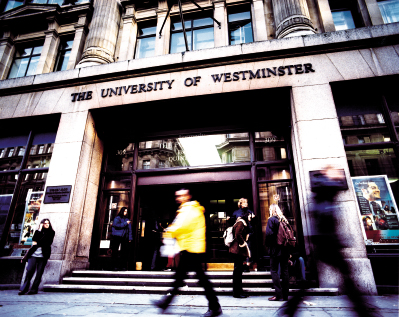
\includegraphics[width=0.9\textwidth]{img/wmin2.jpg}
  \caption{Le campus principal}
\end{figure}
TODO completer pr�sentation

\subsection{Campus et �coles}
L'Universit� de Westminster est actuellement compos� de 6 sites r�partis
dans Londres et ses environs.
\begin{itemize}

\item Le site Cavendish qui se trouve au 101-115 New Cavendish Street
proche de la tour de la British Telecom. Il contient deux �coles :
\begin{itemize}
\item Sciences de la vie
\item Electronique et informatique
\end{itemize}

C'est dans ce site que mon stage s'est d�roul� au sein de l'�cole �lectronique
et Informatique School of electronics and computer science. La figure
suivante pr�sente le b�timent vu de devant.

\begin{figure}[h!]
  \centering
      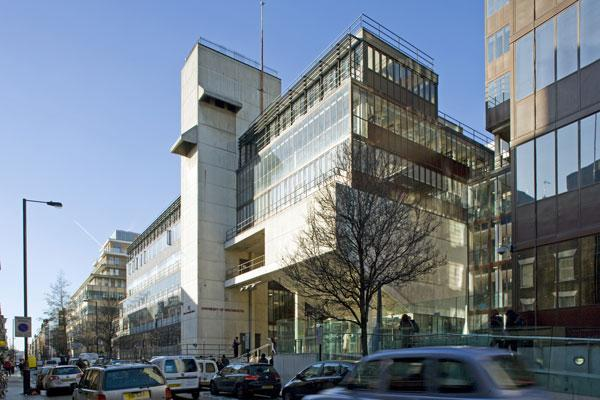
\includegraphics[width=0.9\textwidth]{img/wmin1.jpg}
  \caption{Le campus de New Cavendish Street}
\end{figure}

\item Le site de Great Portland Street se trouve au 70-74 Great Portland
street, il contient le d�partement du centre informatique pour personnes
handicap�es.
\item Le site de Harrow se trouve � Watford road. Il contient deux �coles :

\begin{itemize}
\item une partie de l'�cole d'�lectronique et informatique
\item l'�cole des m�dias, de l'art et du design
\end{itemize}

\item Le site de Little Titchfield Street se trouve au 4-12 Little Titchfield
street, il contient l'�cole de droit.
\item Le site de Marylebone se trouve au 35 Marylebone road. Il contient
l'�cole d'architecture et de construction environnementale.
\item Le site de Regent Street qui se trouve au 309 Regent street est le plus
ancien site de l'universit�. Il comprend l'�cole des sciences sociales, des
sciences humaines et des langues.
\end{itemize}


\subsection{School of Electronics and Computer Science}
Cette �cole est en cohabitation avec l'�cole de sciences de la vie au
sein du site de Cavendish. On peut voir que cette �cole est constitu�e de
d�partements et de 4 groupes de recherches dont voici les �nonces :
\begin{itemize}
\item Department of Business Information Systems
\item Department of Computer Science and Software Engineering
\item Department of Electronic, Network and Computer Engineering
\item Electronic and Communication Engineering
\item Operational Research and Intelligent Systems
\item Parallel and Distributed Computing
\item Semantic Computing and Systems Engineering
\end{itemize}
Cette �cole est tr�s r�put�e pour les programmes d'�changes internationaux.
J?ai pu y d�couvrir nombre d'�tudiants �trangers qui viennent �tudier
dans ce site.
L'�cole propose beaucoup de domaines d'enseignement dans le parcours
informatique. Il est ainsi possible de suivre des cours de gestion de syst�mes
d'information, de programmation parall�le et distribu�e, de programmation
d'intelligence artificielle en passant �galement par le d�veloppement de jeux
vid�os et d'autres formations.


\subsection{Informations et chiffres}

Avec un peu plus de 24000 �tudiants, l'universit� de Westminster fait partie des universit� les plus prestigieuses du Royaume Uni.
L'universit� compte quelques dipl�m�s de prestiges, avec des grands nom tel que Cherie Blair, senior barrister, femme de Tony Blair,
TO DO, Completer cette partie
 




\clearpage
\chapter{Pr�sentation du sujet}
\section{Le projet Yuukou}
\subsection{Pr�sentation}

Yuukou, du japonais qui d�signe la validit� (e), la disponibilit�, l'efficacit�, est un syst�me qui recueille des informations d'authentification � partir de serveurs LDAP afin de comprendre et de construire l'infrastructure des ressources et permet de facilit� son utilisation. Yuukou est �t� cr�� pour faciliter l'utilisation des laboratoires informatiques � l'Universit� de Westminster.





\clearpage
\chapter{Cahier des charges}



\clearpage
\chapter{Organisation et Sp�cifications}

\section{Gestion du temps}

\section{Syst�me d'exploitation}

\section{Mat�riel et Logiciels}

\subsection{Netbeans}

NetBeans est un environnement de d�veloppement int�gr� (IDE\protect\footnote{Interface De D�veloppement}), plac� en open source par Sun en juin 2000 sous licence CDDL et GPLv2. En plus de Java, NetBeans permet �galement de supporter diff�rents autres langages, comme Python, C, C++, JavaScript, XML, Ruby, PHP et HTML. Il comprend toutes les caract�ristiques d'un IDE moderne (�diteur en couleur, projets multi-langage, refactoring, �diteur graphique d'interfaces et de pages Web).
Con�u en Java, NetBeans est disponible sous Windows, Linux, Solaris (sur x86 et SPARC).

NetBeans propose diff�rents outils pour l'exploitation de web services. Il supporte JAX-WS services, JAX-RS RESTful Web Services, standards JAX-RPC Web Service, SOAP et RESTful Web Services. Il permet l'utilisation des web services Google Maps, Yahoo News Search.
Nous l'avons donc utilis� afin de pouvoir acc�der de mani�re simple et efficace aux Web-service mis en place par l'universit� afin de pouvoir acc�der aux informations disponibles.


\subsection{Mozilla et cie}

Mozilla Firefox est un navigateur Web libre et gratuit, d�velopp� et distribu� par la Mozilla Foundation avec l'aide de centaines de b�n�voles gr�ce aux m�thodes de d�veloppement du logiciel libre/open source\protect\footnote{La d�signation open source s'applique aux logiciels dont la licence respecte des crit�res pr�cis�ment �tablis par l'Open Source Initiative, c'est-�-dire la possibilit� de libre redistribution, d'acc�s au code source et aux travaux d�riv�s.} et � la libert� du code source.

Les nombreux plugins ainsi que les outils d'analyse que propose ce navigateur m'ont permis de debbuger mon code.
Plus particuli�rement Firebug, qui m'a permit d'analyser les ent�tes de mes requ�tes a mon Servlet, ainsi que les temps de r�ponses de celui, plus l'�dition du code source et du Javascript.

\subsection{Github}

GitHub est un service web d'h�bergement et de gestion de d�veloppement de logiciels, utilisant le programme Git.

Le site de dit de "\textit{Social Coding}\protect\footnote{Code source libre service}" permet a tout d�veloppeur d'avoir une aide tout au long du d�veloppement de son projet, gr�ce a la gestion de version que celui ci propose.
Cet outil suis l'�volution des fichiers source et garde les anciennes versions de chacun d?eux.

L'utilisation de ce service m'a permit d'avoir un aper�u de l'avancement de mon projet, ainsi que l'affichage de plusieurs statistiques en tout genre.
Cela m'a �galement permit d'avoir une copie de mon travail sur un serveur distant en cas de crash de ma machine.

Il existe plusieurs types de logiciels proposant le m�me type de service comme SVN, Mercurial, CVS ... Mais Git m'a sembl� le plus appropri� et le plus facile a prendre en main.

Ces logiciels sont fortement conseill�s pour g�rer un projet informatique.

\section{Les langages}
\subsection{JAVA}

Le langage Java est un langage de programmation informatique orient� objet cr�� par James Gosling et Patrick Naughton, employ�s de Sun Microsystems.
Ses caract�ristiques ainsi que la richesse de son �cosyst�me et de sa communaut� lui ont permis d'�tre tr�s largement utilis� pour le d�veloppement d'applications de types tr�s disparates. Java est notamment largement utilis� pour le d�veloppement d'applications d'entreprise et mobiles.
Apr�s les plusieurs essai infructueux avec PHP, j'ai d�cid� de basculer sur le langage JAVA qui m'a grandement facilit� la tache, aussi gr�ce a la communaut� tr�s active sur le web.
En effet la communication a un serveur en utilisant certaines strat�gie de s�curit� comme SSL\protect\footnote{\textit{Secure Sockets Layer}, un protocole de s�curisation des �changes sur Internet} et bien plus simple en JAVA. L'IDE r�cup�re le certificat et le signe avec l'accord de l'utilisateur.
Protocole efficace et simplifi� par rapport � celle utilis�e en PHP, que nous d�velopperons dans la partie des probl�mes rencontr�s


\subsection{JavaServer Pages}

Le JavaServer Pages ou JSP est une technique bas�e sur Java qui permet aux d�veloppeurs de cr�er dynamiquement du code HTML, XML ou tout autre type de page web. Cette technique permet au code Java et � certaines actions pr�d�finies d'�tre ajout�s dans un contenu statique. Depuis la version 2.0 des sp�cifications, la syntaxe JSP est compl�tement conforme au standard XML.
En clair, un fichier JSP g�n�re du code HTML, en effectuant les actions d�finies par le code JAVA qui est contenu dans les balises not�es "<%%>".
En r�cup�rant les informations que le Servlet\protect\footnote{Voir la partie } me renvoi, nous effectuons les traitements sur les objets r�cup�r�s.
En regardant le code source de la page, elle apparait comme une page HTMl statique.

\section{Formats de donn�es}

\subsection{JavaScript Object Notation}

JavaScript Object Notation ou plus commun�ment appel� JSON est un format de donn�es textuel et g�n�rique. Il permet de repr�senter de l?information structur�e.
Un document JSON ne comprend que deux �l�ments structurels :
\begin{itemize}
    \item des ensembles de paires nom / valeur
    \item des listes ordonn�es de valeurs.
\end{itemize}

Ces m�mes �l�ments repr�sentent 3 types de donn�es :
\begin{itemize}
\item  des objets
\item  des tableaux
\item  des valeurs g�n�riques de type tableau, objet, bool�en, nombre, cha�ne ou null.
\end{itemize}

Pourquoi JSON ?
Tout simplement parce que JSON est plus l�ger, et beaucoup plus rapide a interpr�ter que XML.
Sur des un certain nombre de donn�es, la diff�rence est flagrante, JSON est beaucoup plus rapide XML.
C'est suite a un besoin de performance que nous avons opt� pour le JSON.

\begin{figure}[h!]
  \centering
      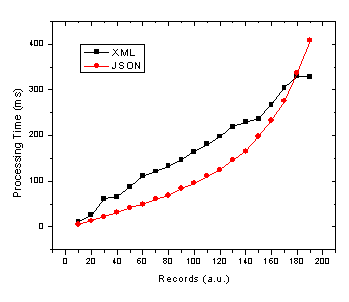
\includegraphics[width=0.9\textwidth]{img/jsonxml.png}
  \caption{Performance mesur�e entre JSON et XML}
\end{figure}


\section{Frameworks et Libraires}

\subsection{jQuery Mobile}

jQuery Mobile est un framework\protect\footnote{un framework est un kit de composants logiciels} web optimis�e pour Smart-phones actuellement d�velopp� par l'�quipe du projet jQuery. Le d�veloppement se concentre sur la cr�ation d'un framework compatible avec une grande vari�t� de smart-phones et tablettes, chose rendue indispensable a cause de l'explosion des march� des plateformes mobiles.
Gr�ce a ce framework, nous avons pu cr�e la partie client de \textbf{Yuukou2}, de mani�re simple intuitive, et optimis� pour les plateformes mobiles.


\subsection{Google Chart API}

Le API Google Chart est un outil qui permet aux gens de cr�er un graphique � partir de certaines donn�es et de l'int�grer dans une page web. Google cr�e une image interactive � partir des donn�es ins�r�s dans le tableau. De nombreux types de graphiques sont pris en charge.
\begin{figure}[h!]
  \centering
      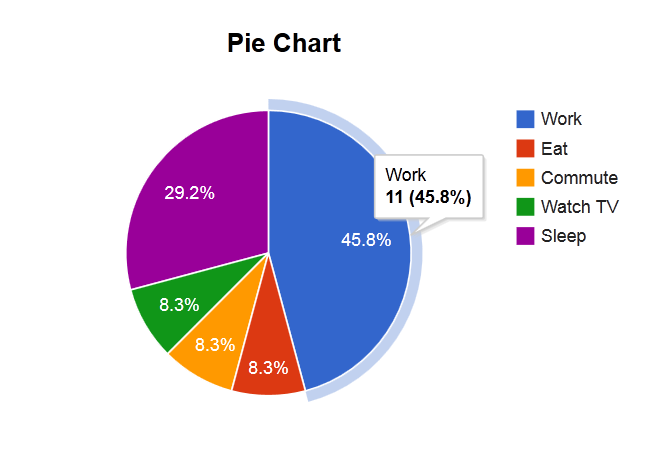
\includegraphics[width=0.9\textwidth]{img/googleapi.png}
  \caption{Exemple d'affiche d'un diagramme de statistique avec Google API}
\end{figure}

 De tableaux en ligne simples � carte complexes d'arbres hi�rarchiques, la galerie fournit un grand nombre de types de graphiques bien con�us. 


\subsection{JFreeChart}
JFreeChart est une API Java permettant de cr�er des graphiques et des diagrammes de tr�s bonne qualit�. Cette API est open source et sous licence LGPL.
Cet outils permet de generer des graphique statitiques, qui seront sauvegarger en fichier image, ce qui rend utilie la recup�ration des donn�es a une date donn�e.



\clearpage

\end{document}

